\documentclass{standalone}
\usepackage{multicol}
\usepackage{tikz}
\usetikzlibrary{calc,angles,positioning,intersections,quotes,decorations.markings}
\usepackage{tkz-euclide}
\usetkzobj{all}
\usepackage{pgfplots}
\pgfplotsset{compat=1.16}

\begin{document}
	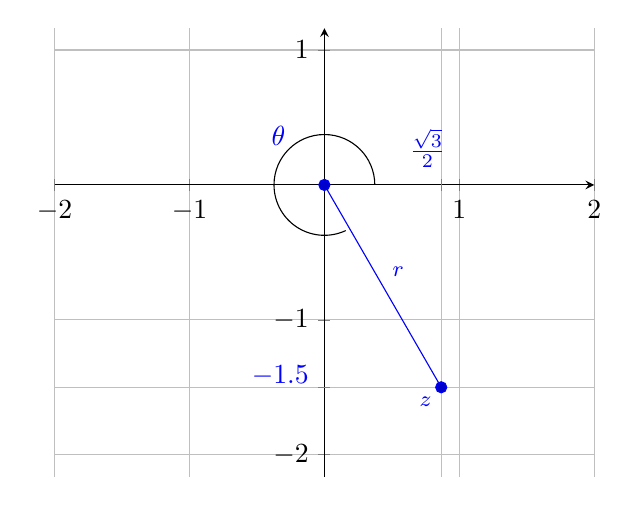
\begin{tikzpicture}
		\begin{axis}[axis lines=middle, axis equal, grid=both, xmin=-2, xmax=2, ymax=1, ymin=-2, 
						extra x ticks={sqrt(3)/2}, extra x tick style={tick label style={yshift=6ex, xshift=-0.5em, blue}}, extra x tick labels={{$\frac{\sqrt{3}}{2}$}}, 
						extra y ticks={-1.5}, extra y tick style={tick label style={yshift=1ex, blue}}]
			\addplot coordinates {(0,0) ({sqrt(3)/2}, -1.5)}
				node[below left,pos=1,font=\footnotesize](Z){$z$}
				node[above right,pos=0.5,font=\footnotesize]{$r$};
			\addplot+[no marks]
				({sqrt(3)/2}, 0) node[fill=none, draw=none] (X){};
			\addplot+[no marks]
				(0, 0) node[fill=none, draw=none] (start){};
		\end{axis}
		
		\tkzMarkAngle[scale=0.8](X,start,Z)
		\draw (start) node[above left=1.5em, blue]{$\theta$};

	\end{tikzpicture}
\end{document}